\documentclass{beamer}
\usetheme{Madrid}
\usecolortheme{default}


\usepackage[T1]{fontenc}
\usepackage[utf8]{inputenc}
\usepackage{amsmath,amssymb,bm,mathtools}
\usepackage{xcolor}
\usepackage{hyperref}
\usepackage{microtype}

\graphicspath{{./figures/}}
\usepackage{booktabs}


\title[Project 2]{Project 2}
\subtitle{CS 332, Fall 2025}
\author{Ben Cole \and Koshi Harashima}
\date{22 October, 2025}

\begin{document}

\maketitle

\begin{frame}{Outline}
  \tableofcontents
\end{frame}

%===================== we can skip this section! ==========================================
\section{Basic Setting}

\begin{frame}{Basic Setting - Online Learning}
    \textbf{Online Learning}: 
    \begin{itemize}
        \item k actions
        \item n rounds
        \item action $j$'s payoff in round i ; $v_j^i \in [0,h]$
        \item in round i:
        \begin{itemize}
            \item choose an action $j^i$
            \item learn payoffs $v_1^i, \dots, v_k^i$
            \item obtain payoff $v_j^i$
        \item Payoff $ALG = \sum_{i = 1} ^n v_j^i$
        \item the best in hindsight payoff is 
        \[
        OPT = max_j \sum_{i = 1} ^n v_j^i
        \]
        \item the regret of the algorithm is 
        \[
        Regret_n = \frac{1}{n}[OPT - ALG]
        \]
        \end{itemize}
    \end{itemize}
\end{frame}

\begin{frame}{Basic Setting - Exponential Weights Algorithm}
    \textbf{Exponential Weights Algorithm}\\[3pt]
    \begin{itemize}
        \item Learning rate: $\epsilon$
        \item In round $i$, choose action $j$ with probability $\pi_j^i$ defined by
        {\scriptsize
        \[
            \pi_j^i = 
            \frac{(1+\epsilon)^{\frac{V_j^{i-1}}{h}}}
            {\sum_{j'} (1+\epsilon)^{\frac{V_{j'}^{i-1}}{h}}}
        \]
        }
    \end{itemize}

    \vspace{2pt}
    \textbf{Regret Bound} (Discussed in Exercise)\\[3pt]
    \[
    \mathrm{Regret}_n 
    = 
    \max_j \sum_{i=1}^{n} v_j^i 
    - 
    \mathbb{E}\!\left[\sum_{i=1}^{n} v_{a_i}^i\right]
    \;\le\;
    \epsilon n h + \frac{h \log k}{\epsilon}
    \]
    When $\epsilon$ is set optimally as 
    $\epsilon = \sqrt{\frac{\log k}{n}}$, we have
    \[
    \mathrm{Regret}_n \;\le\; 2h\sqrt{n \log k}.
    \]
\end{frame}


\begin{frame}{Basic Setting - MC Simulation}
    \textbf{Monte Carlo Simulation}\\
    we implemented MC Simulation as follows:
    \begin{itemize}
        \item fix k, n, the number of iteration
        \item for each run, 
        \begin{enumerate}
            \item set $\epsilon$ to {$0.01, \sqrt{log\frac{k}{n}}, 100$}
            \item Simulate it using the implemented algorithms for each setting.
            \item calculate Regret
        \end{enumerate}
        \item calculate mean and their confident intervals.
    \end{itemize}
    \textbf{Learning Rates}\\
    \begin{itemize}
      \item No learning: \(\epsilon = 0\) .
      \item Theoretical: \(\epsilon = \sqrt{\ln k / n}\).
      \item FTL:  \(\epsilon \approx \infty\).
    \end{itemize}
\end{frame}

\begin{frame}{Basic Setting - Appendix}
    FTL is defined as follows:
    \begin{itemize}
        \item $V_j^i = \sum_{r=1}^i v_j^r$
        \item in round i , choose $j^i = argmax_j V_j^i$
    \end{itemize}
    uniform guessing is defined as follows:
    \begin{itemize}
      \item in round i, choose j randomly.
    \end{itemize}
\end{frame}

% \begin{frame}{Basic Setting - Summary}
%     In each part, we show 4 things
%     \begin{enumerate}
%         \item Game settings
%         \item Their structure and our intuition of results
%         \item The change of Regret in rounds(Regret bound of optimal learning rate)
%         \item The change of total payoffs in rounds
%     \end{enumerate}
%     we will describe some observations from the analysis of comparative statics (changing parameters). 
% \end{frame}
%===================== we can skip this section! ==========================================

\section{Part 1}
\begin{frame}{Part 1 - Outline}
In Part 1, we consider two things;
\begin{enumerate}
    \item Adversarial Fair Payoffs (hereinafter abbreviated as "AFP") 
    \item Bernoulli Payoffs (hereinafter abbreviated as "BP")
\end{enumerate}
\end{frame}

\begin{frame}{Part 1 - Summary}

\textbf{Methods}\\
In AFP and BP, we first gain intuition from observation, then simulate them.
\vspace{1em}

\textbf{Results}\\
In AFP, FTL works poorly, while other learning rates work well.\\
In BP, FTL works better than the others.
\vspace{1em}

\textbf{Takeaways}\\
FTL performs best in an environment where there is an optimal arm. Random and optimal learning rates perform best in an environment without an optimal arm.

\end{frame}

\subsection{A: AFP}

\begin{frame}{A - Setting}
    In each round i:
    \begin{itemize}
        \item Draw a payoff $x \sim U[0,1]$
        \item If there are several actions whose total payoff is zero, payoff is randomly assigned to these actions.
        \item Assign this payoff to the action $j^*$ that has the smallest total payoff so far,\\
        i.e., $j^* = \arg\min_j V^{i-1}_{j} \quad \text{where} \quad V^{i}_{j} = \sum_{r=1}^{i} v^{r}_{j}$
    \end{itemize}
    \vspace{1em}
    Here are the fixed parameters we used;
    \begin{itemize}
        \item k = 3
        \item n = 1000
    \end{itemize}
\end{frame}

\begin{frame}{A - Game structure and Intuition}
    Our intuition is that
    \begin{itemize}
        \item FTL will work poorly because the more aggressively one seeks to maximize profit in this setting, the lower the realized profit.
        \item Since payoffs are drawn from uniform distribution, we can't predict the cumulative payoff for each arm. This is why random/optimal should perform well.
    \end{itemize}
    \begin{figure}
        \centering
        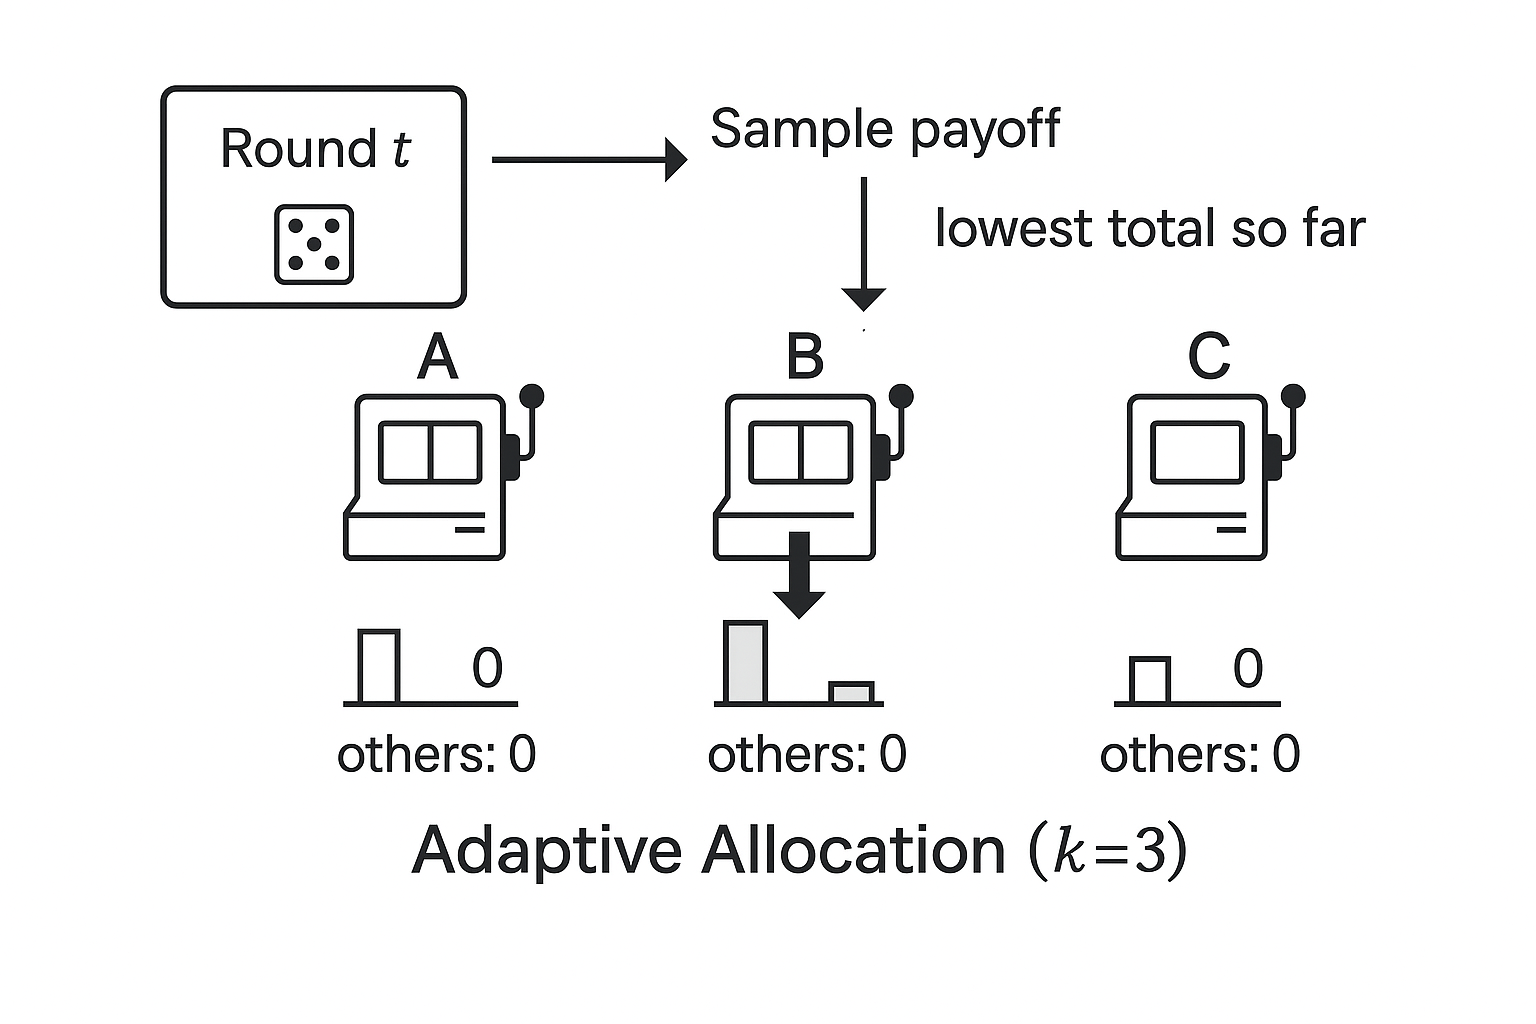
\includegraphics[width=0.5\linewidth]{../figures/Image_A.png}
        \label{fig:placeholder}
    \end{figure}
\end{frame}

\begin{frame}{A - Results (Regret)}
Here is a graph showing the change in regret. \\
We conclude that these results are consistent with the intuition.
\begin{itemize}
    \item FTL regret increases linearly in rounds
    \item Random/optimal $\epsilon$ regret stays almost zero.
\end{itemize}
\begin{center}
    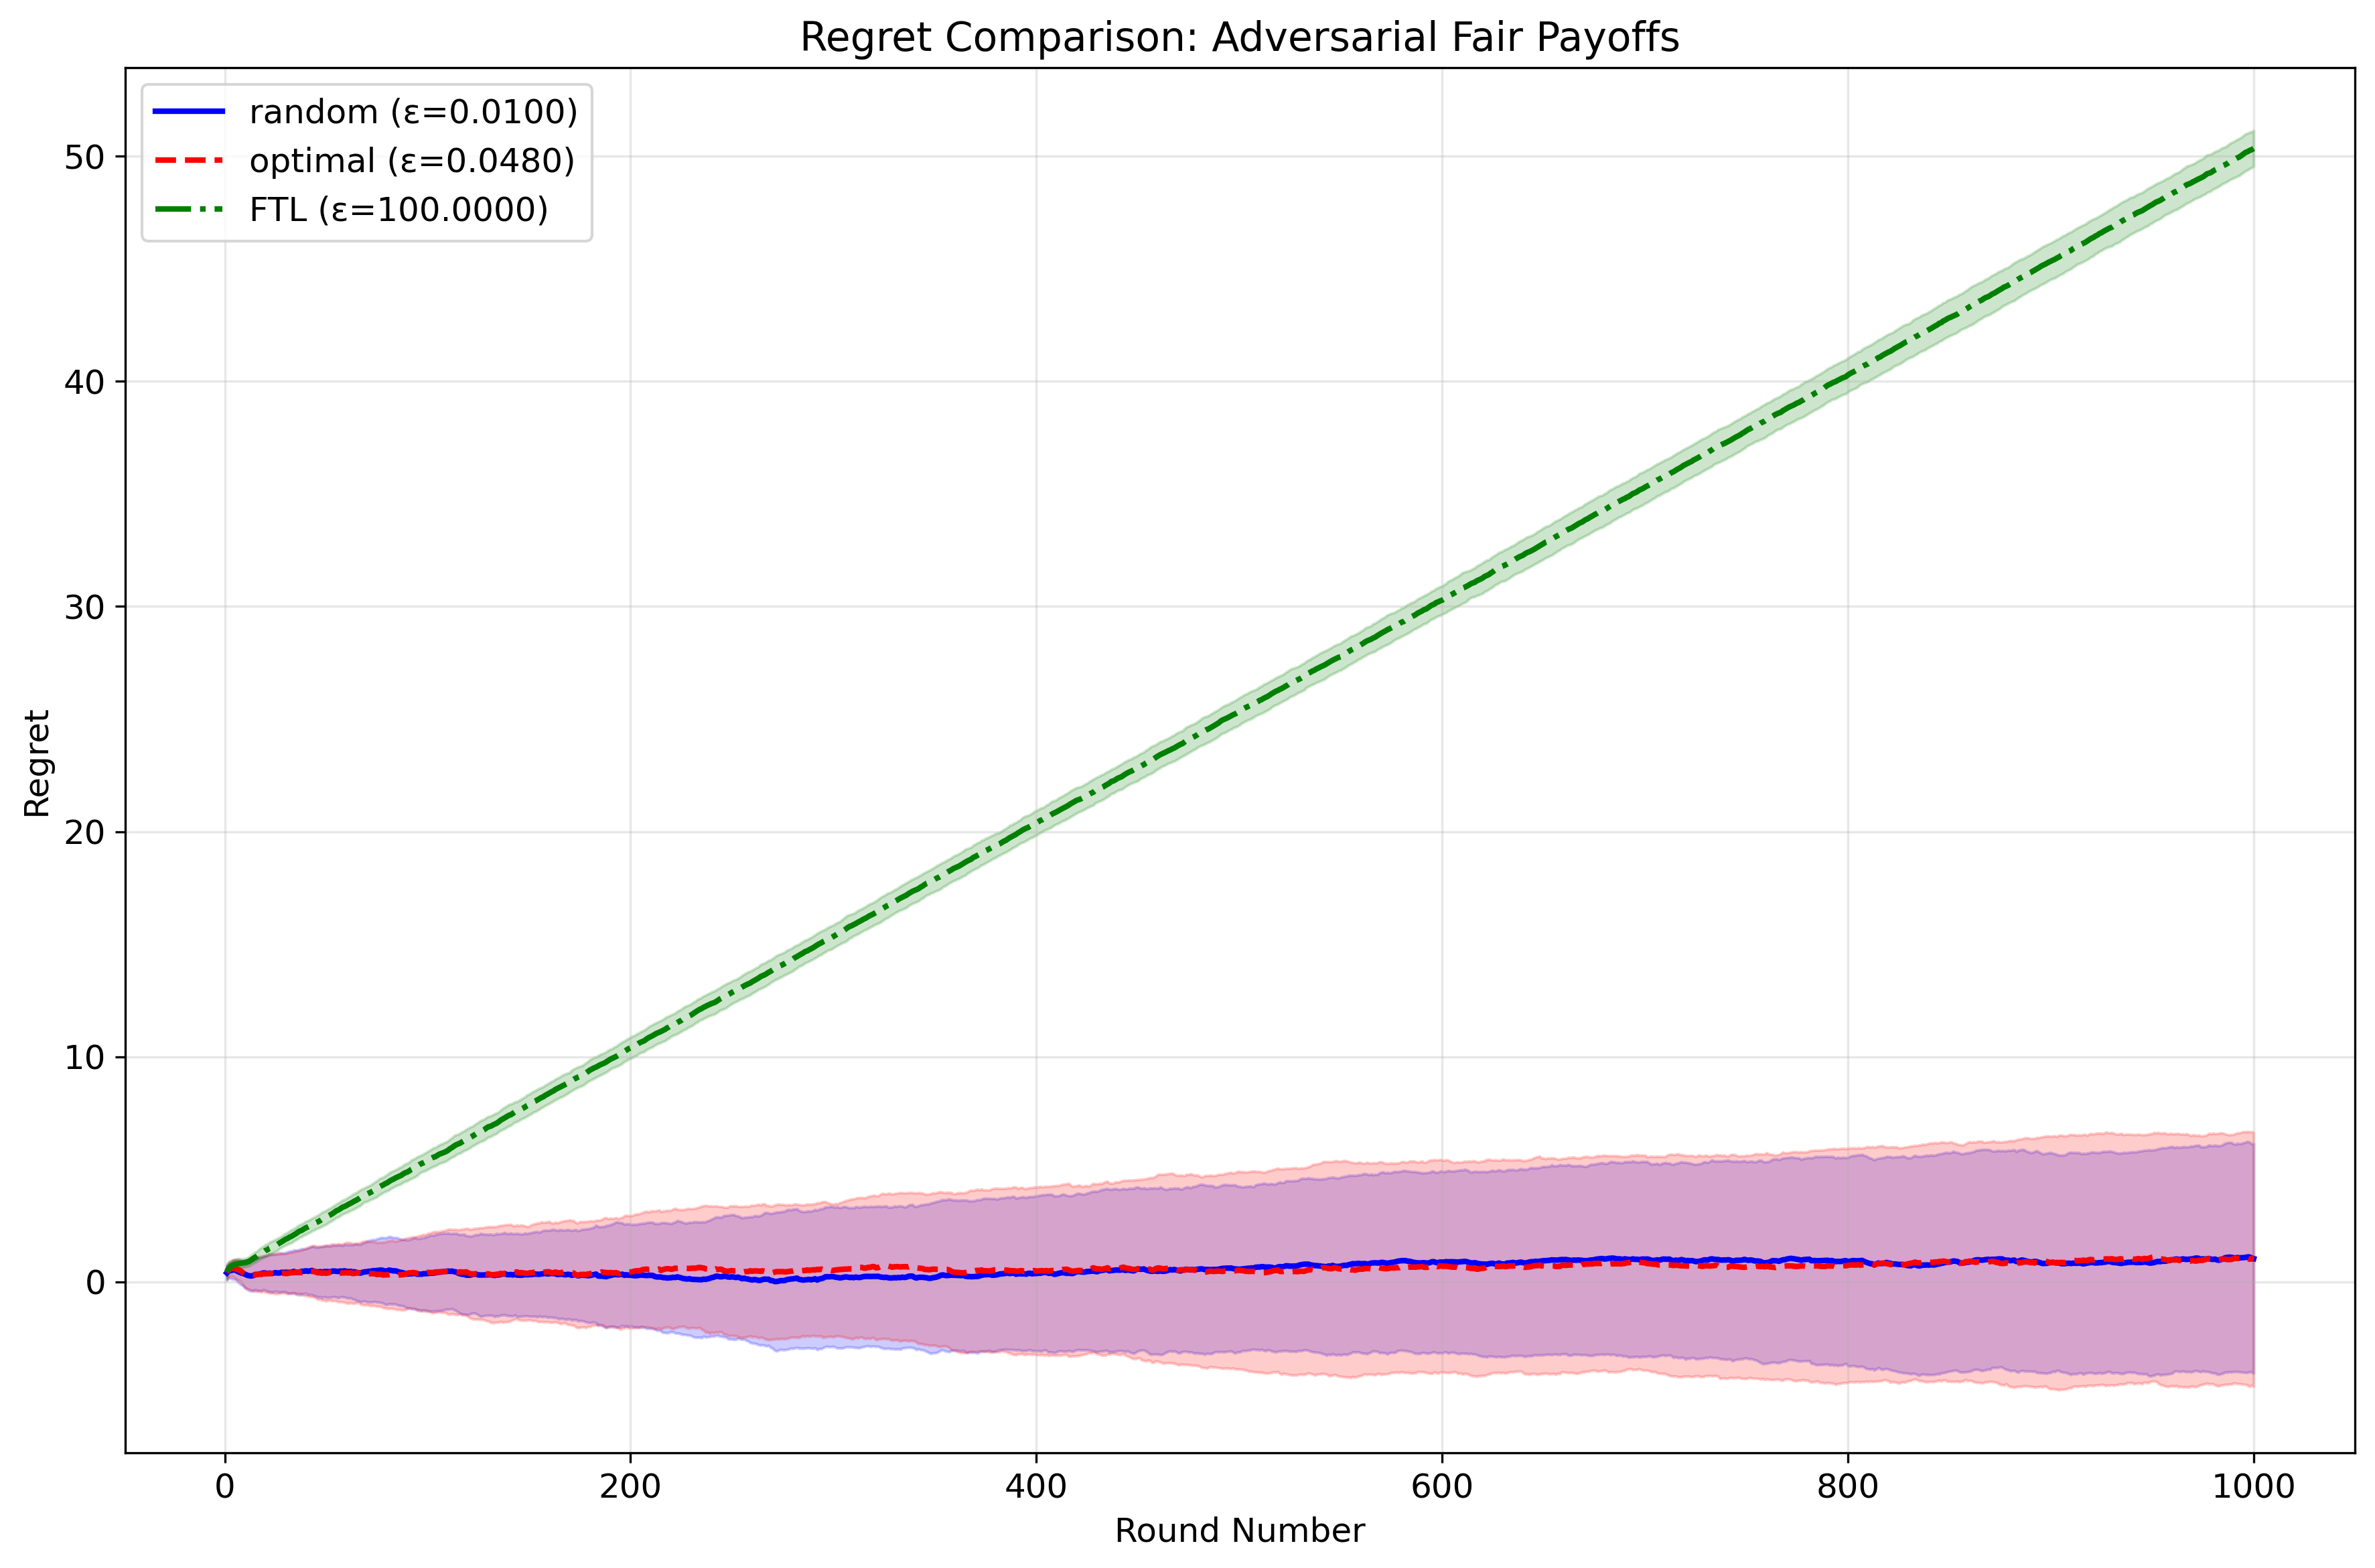
\includegraphics[width=0.7\textwidth]{../figures/adversarial_regret_comparison.png}
\end{center}
\end{frame}

% \begin{frame}{A - Additional Analysis on Results}
% \textbf{FTL}\\
% Each round, FTL regrets what he did. Then, he chooses the action whose total payoff in past is the most. We know this "previously optimal" action will point to O in the next round, which explains why he never wins, and his regret increases linearly.
% \textbf{random}\\
% \textbf{optimal}\\
% \end{frame}

\begin{frame}{A - Results (Payoffs)}

\begin{figure}
    \centering
    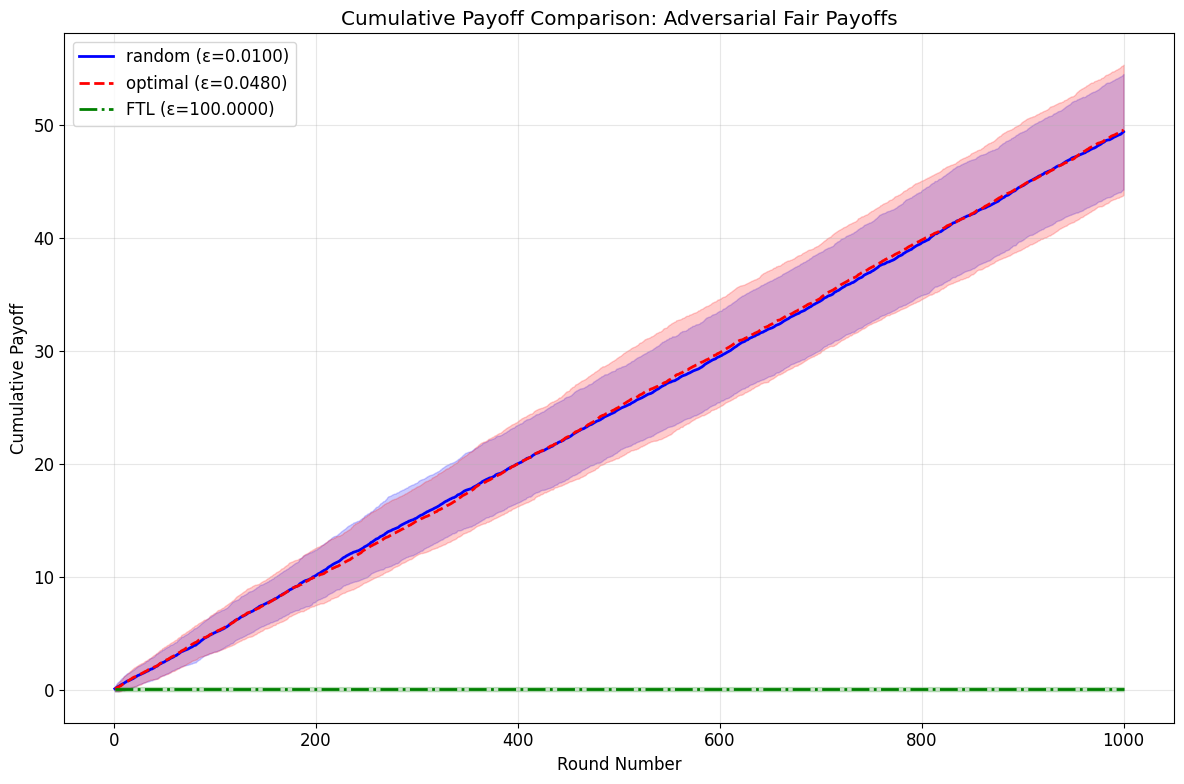
\includegraphics[width=0.8\linewidth]{figures/AFR_payoff.png}
    \caption{Payoff}
    \label{fig:placeholder}
\end{figure}

\end{frame}

\begin{frame}{A - Results (Regret Bound)}
According to the setting, regret bound for optimal learning rate is
\[Regret_t \leq 2 * 1 * \sqrt{1000log3} \approx 110\]
We can easily see that regret is binded by this bound.
\end{frame}

\subsection{B : BP}

\begin{frame}{B - Setting}
    Fix a probability for each action $p_{1},...,p_{k}$ with each $p_{k}$ in [0,1/2].\\
    In each round i,
    \begin{itemize}
        \item draw the payoff of each action j as $v^{i}_{j} \sim B(p_{j})$ (i.e, from the Bernoulli distribution with probability $p_j$ of being 1 and probability $1-p_{j}$ of being 0).
        \item full-information(no Bandit)
    \end{itemize}
    \vspace{1em}
    Here's our parameters;
    \begin{itemize}
        \item k = 3
        \item n = 1000
    \end{itemize}
\end{frame}

\begin{frame}{B - Game structure and Intuition}
    Our intuition is that 
    \begin{itemize}
        \item since probabilities are fixed, FTL will find the best machine with highest probability earliest
        \item optimal will slowly approach toward the best machine
        \item random will work poorly.
    \end{itemize}
    \begin{figure}
        \centering
        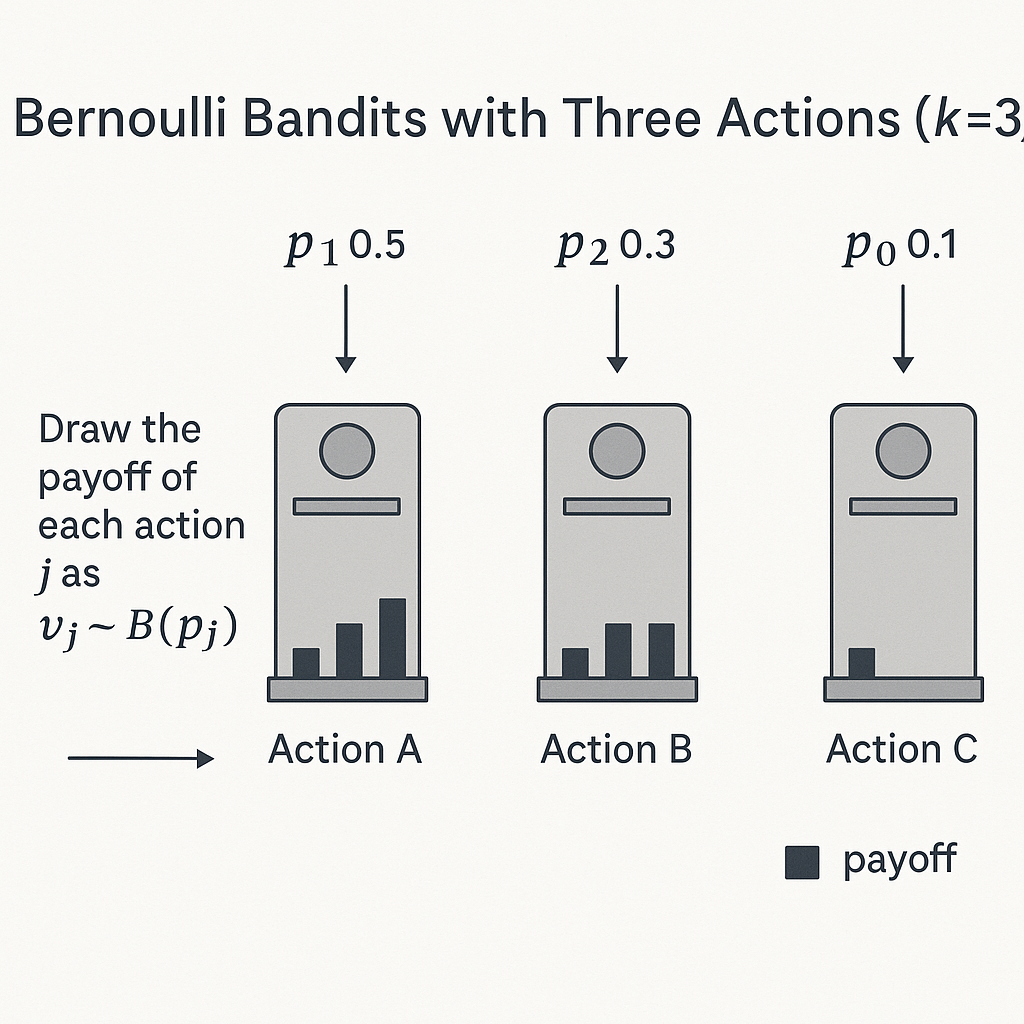
\includegraphics[width=0.4\linewidth]{../figures/Image_B.png}
        \label{fig:placeholder}
    \end{figure}
\end{frame}

\begin{frame}{B - Results(Regret)}
Here is a graph showing the change in regret. \\
We conclude that these results are consistent with the intuition. \\
\begin{center}
    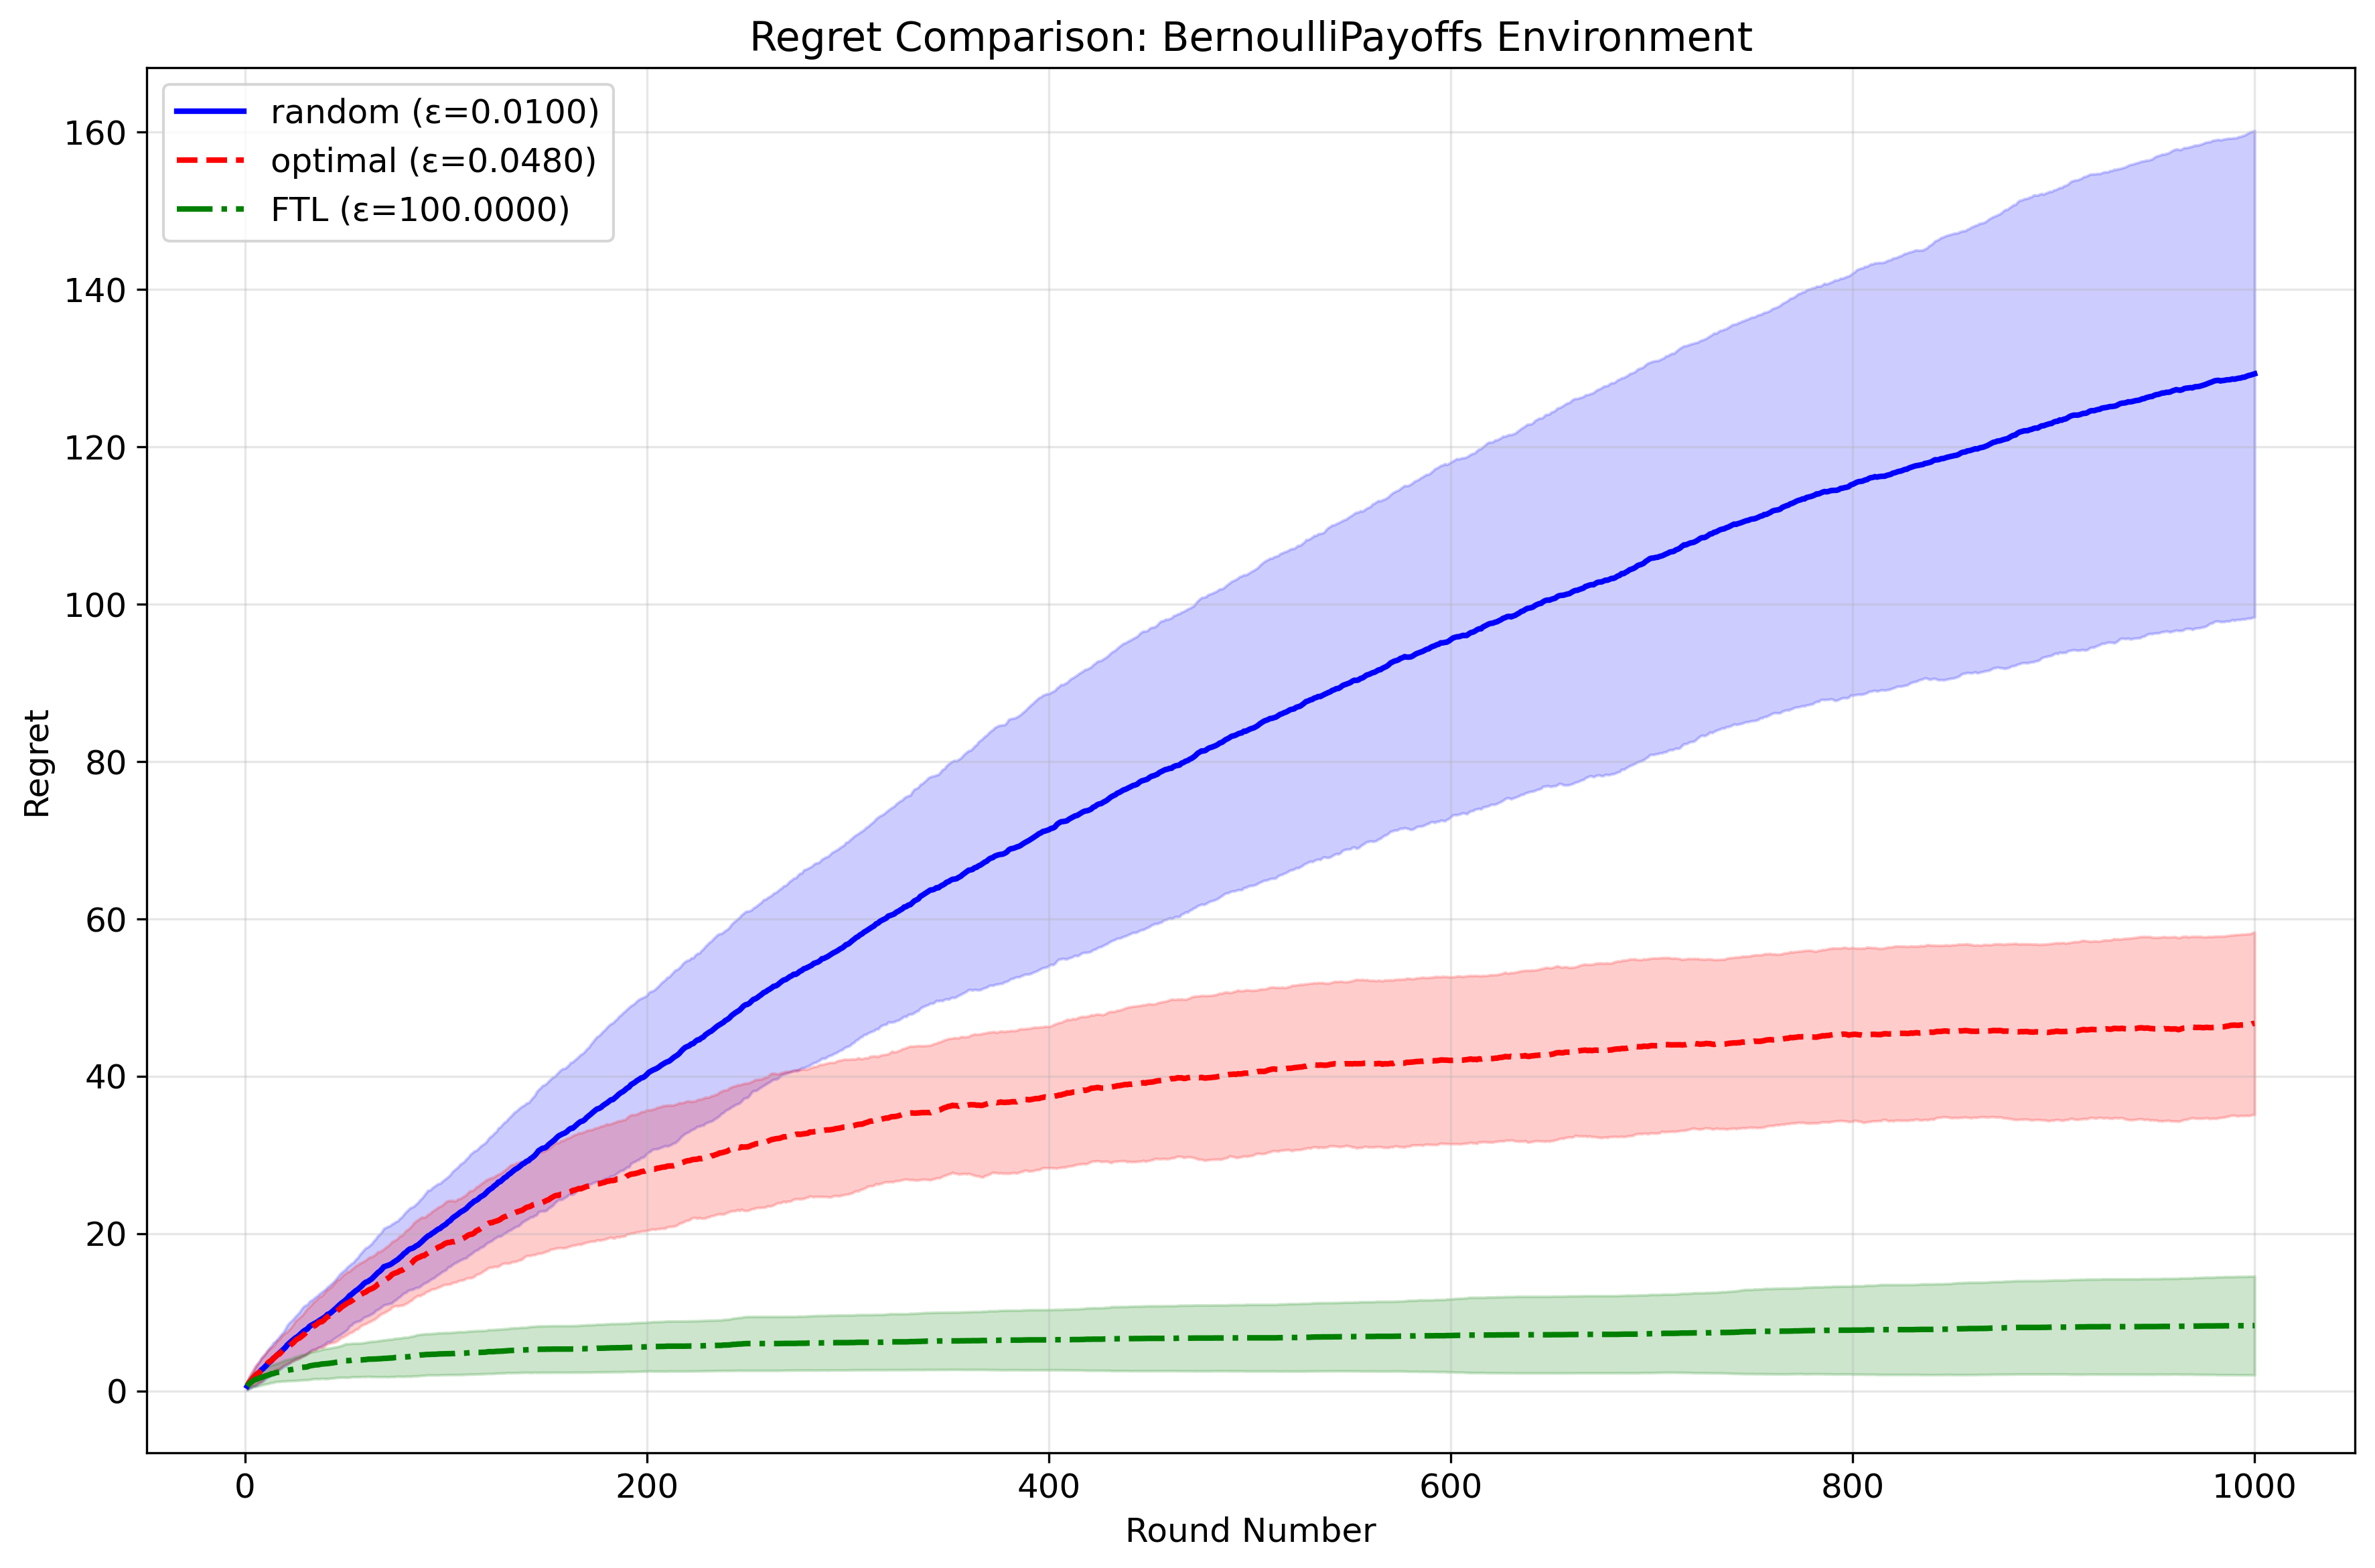
\includegraphics[width=0.8\textwidth]{../figures/bernoulli_regret_comparison.png}
\end{center}
\end{frame}

\begin{frame}{B - Additional Results}
If n increases,  FTL will choose the action which is  optimal choice.
Because FTL has mechanism that choose higheset tota
\[
\frac{\text{total payoff}_j}{\text{rounds}_j} \approx p_j \quad n \rightarrow\infty
\]
which means FTL finds machines with the higest possibility.so not converge to local optima.
\begin{center}
    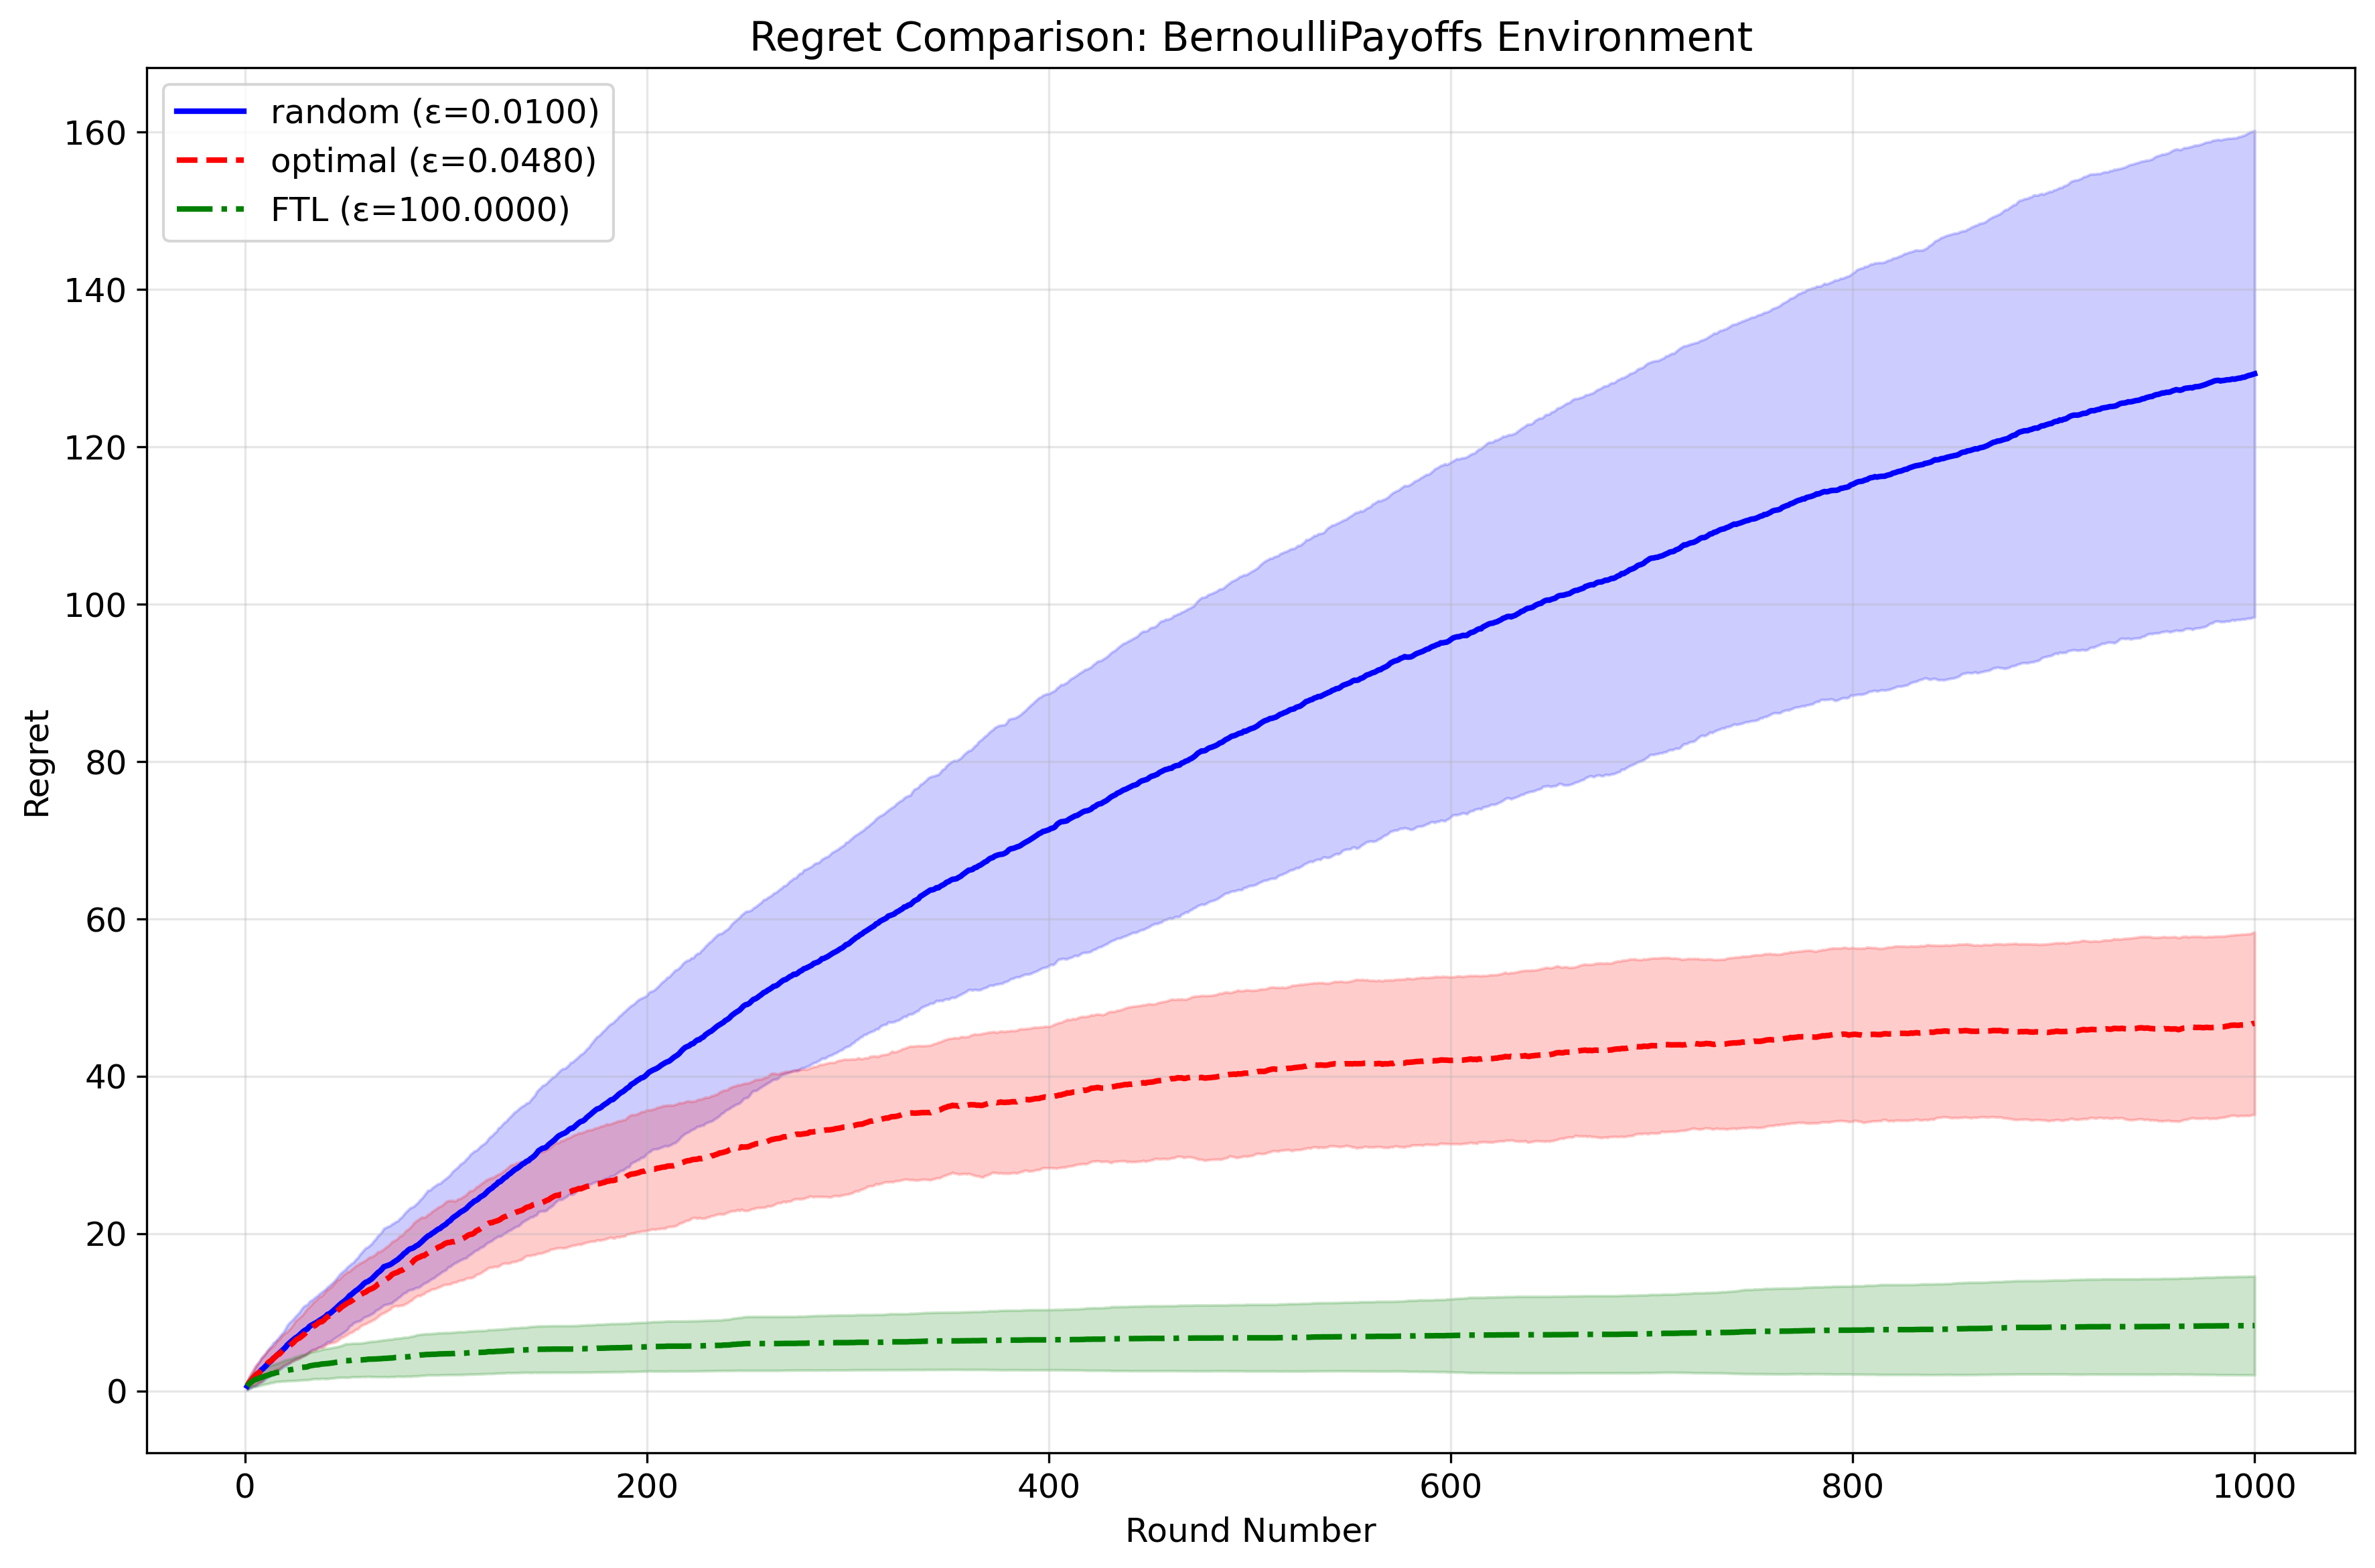
\includegraphics[width=0.5\textwidth]{../figures/bernoulli_regret_comparison.png}
\end{center}
\end{frame}

\begin{frame}{B - Results(Payoffs)}
\textbf{Results}\\
Calculating total payoffs in this setting. it is consistent with result
\begin{center}
    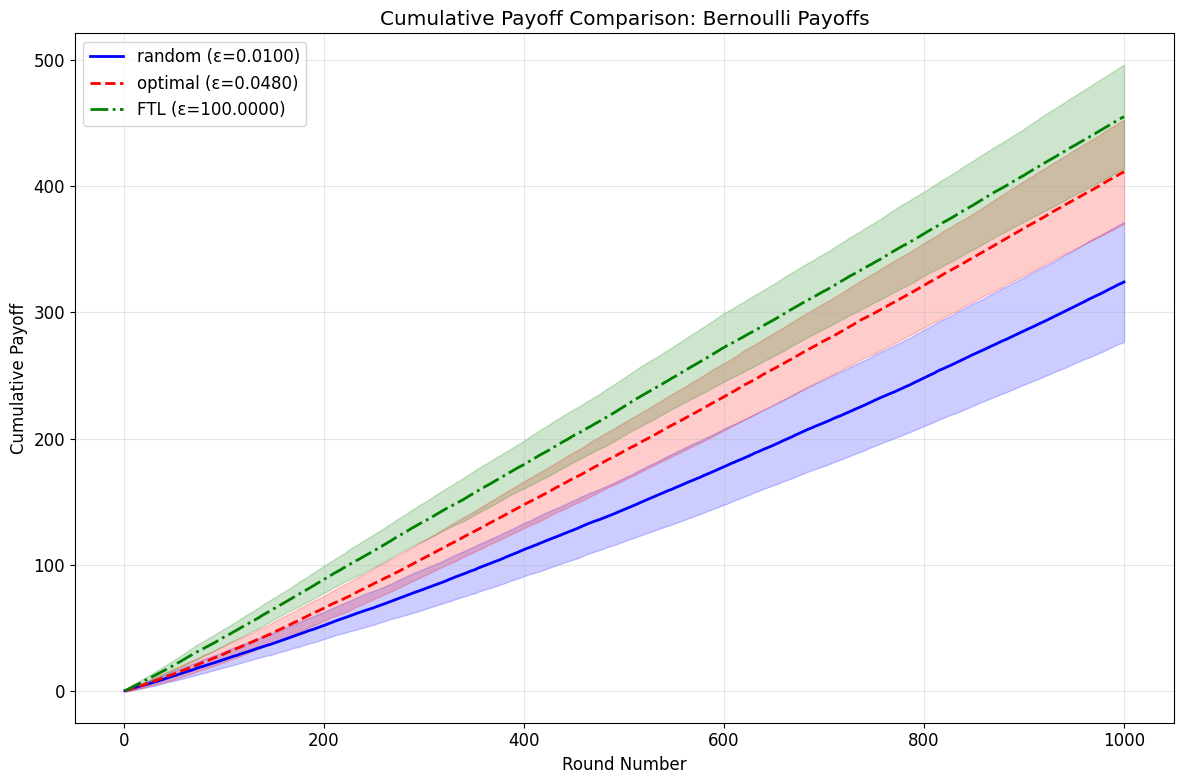
\includegraphics[width=0.5\textwidth]{figures/BP_payoff.png}
\end{center}
\end{frame}

\begin{frame}{B - Results(Regret bound)}
\textbf{Results}\\
    According to the setting, regret bound for optimal learning rate is
    \[
    Regret_t \leq 2 * 1 * \sqrt{1000log3} \approx 110
    \]
\end{frame}


\section{Part2}


\begin{frame}{Part 2 - Outline}
In Part 2, we consider two things;
\begin{enumerate}
    \item Data in the Wild
    \begin{itemize}
        \item EW algorithm applied to Pachinko Payoffs (hereinafter abbreviated as "PP")
        \item we used data from Pachinko
    \end{itemize}
    \item Adversarial Generative Model
    \begin{itemize}
        \item Research Payoffs (hereinafter abbreviated as "RP")
        \item we modeled our Researcher's decision to review the previous researches in online learning framework.
    \end{itemize}
\end{enumerate}
\end{frame}

\subsection{C : PP}

\begin{frame}{C - Summary}
\textbf{Methods}\\
In part C, Using unique data from Japanese Pachinko, and formulate the problem of store selection.  

\vspace{1em}
\textbf{Results}\\
FTL's regret converges to 0, while the others performs poorly.

\vspace{1em}
\textbf{Takeaways}\\
From limited data, we show the optimality of common strategies.
\end{frame}

\begin{frame}{C - Description of Pachinko}
Pachinko is \textbf{a Japanese gambling-like game} that uses small steel balls, which can be exchanged indirectly for money. A pachinko machine can be modeled as a stochastic system that draws payoffs from fixed probabilities, often involving state transitions
\vspace{1em}

While we could not obtain empirical data from actual machine logs on the scale of thousands of plays, we discovered \textbf{another interesting dataset} that captures related dynamics.
\begin{figure}
    \centering
    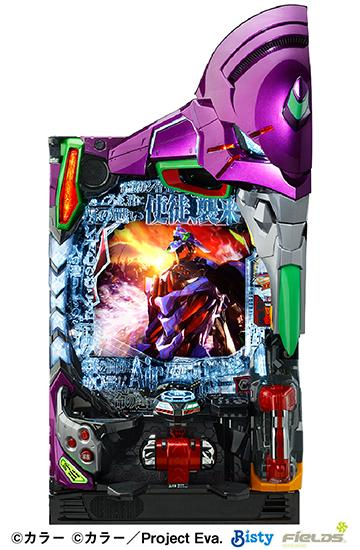
\includegraphics[width=0.15\linewidth]{../figures/machine_evangelion.jpg}
    \caption{Machine Example}
    \label{fig:placeholder}
\end{figure}
\end{frame}

\begin{frame}{C - Description of Data}

Pachinko stores publicly report daily ball counts (in/out), so we can calculate daily average ROI (Return Of Investment) from this data.\\
\vspace{1em}
Two characteristics align with the modeling choice:
\begin{itemize}
  \item \textbf{Aggregation:} Store-level ROI is a coarse proxy for machine-level profitability, but it is observable and comparable across stores day by day.
  \item \textbf{Nonstationarity:} Stores strategically change settings to attract customers or to gain profit, so payoffs can be nonstationary.
\end{itemize}
we choose 5 stores in major cities in Tokyo.
\end{frame}

\begin{frame}{C : Time series of daily ROI}
Below is the time series of daily ROI in each store, showing the nonstationarity characteristic.
\begin{figure}
    \centering
    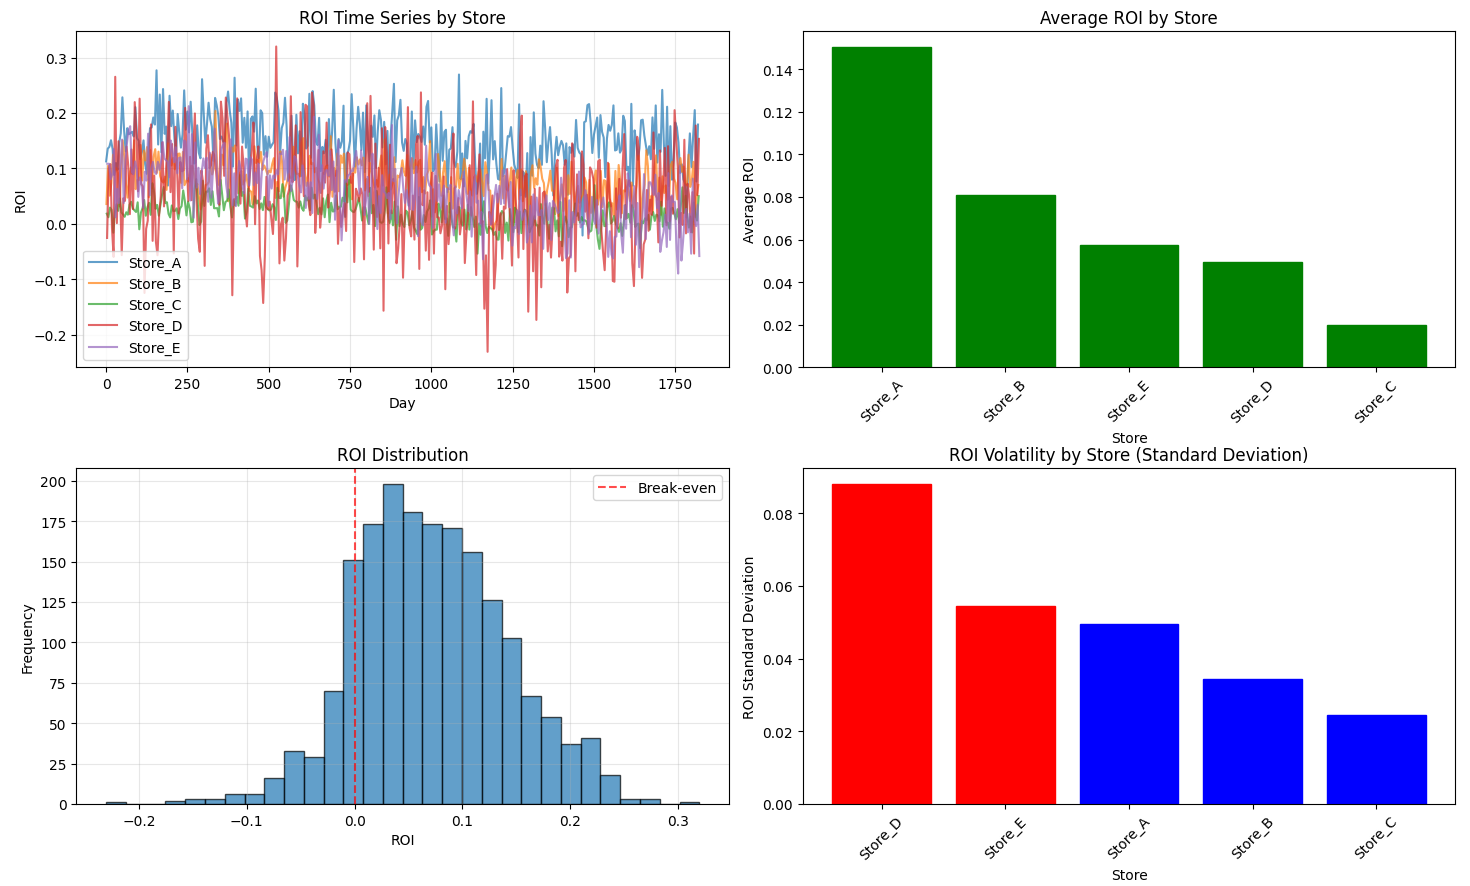
\includegraphics[width=0.8\linewidth]{332Project2/figures/ROI.png}
    \caption{ROI}
    \label{fig:placeholder}
\end{figure}
    
\end{frame}

\begin{frame}{C : Time series of daily ROI}
Below is the time series of daily ROI in each store, showing the nonstationarity characteristic.
    \begin{figure}
        \centering
        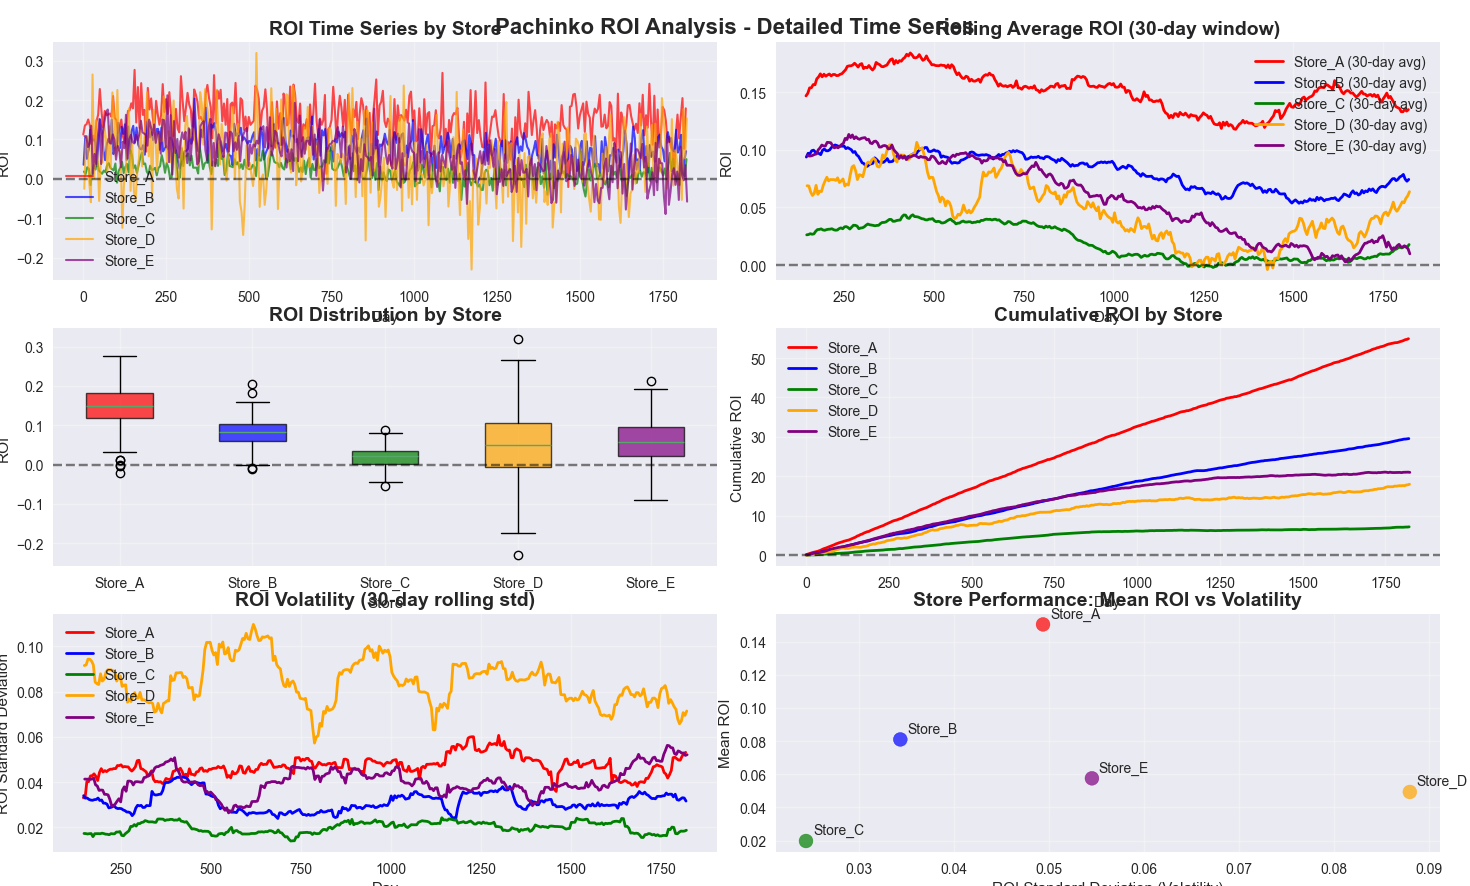
\includegraphics[width=0.8\linewidth]{332Project2/figures/ROI_detailed.png}
        \caption{ROI}
        \label{fig:placeholder}
    \end{figure}
\end{frame}


\begin{frame}{C - Appendix}
    \textbf{Excuse}\\
    This formulation of problem is not far from the real-world strategy. We use data which is trusted among this community in Japan. In addtion, Practitioners often aggregate and forecast store-level returns, sometimes coordinating group play.\\
    This motivates treating each store as an “arm" and applying Exponential Weights Algorithm to store choices rather than to individual machines. 
\end{frame}

\begin{frame}{C - Data}
    Here's how we use data.\\
    \begin{itemize}
        \item \textbf{ROI Data define Payoffs.}\\
    Let stores $s\in\{1,\dots,S\}$ (e.g.\ $S=5$) and days $i=1,\dots,I$.\\
    From data, for each $(s,i)$ observe balls-in/out and total balls:
    \[
    B^{\text{in}}_{s,i},\quad B^{\text{out}}_{s,i},\quad T_{s,i}>0.
    \]
    Define raw ROI and a per-day normalized payoff in $[0,1]$:
    \[
    r_{s,i}\;=\;\frac{B^{\text{out}}_{s,i}-B^{\text{in}}_{s,i}}{ T_{s,i}},\qquad
    v_{s,i}\;=\;\frac{r_{s,i}-\underline r_i}{\overline r_i-\underline r_i+\varepsilon}\in[0,1],
    \]
    where $\underline r_t=\min_{j} r_{j,i}$, $\overline r_i=\max_{j} r_{j,i}$, and $\varepsilon>0$ is small.
    \end{itemize}
\end{frame}

\begin{frame}{C - Setting}
In each day i, Player
\begin{enumerate}
  \item Choose a store $s_i$ 
  \item from data Extract ROI as $v_{s,i}$
\end{enumerate}
\vspace{1em}
So, it's a simple setting of player choosing stores among 5 stores under full-information.

\end{frame}

\begin{frame}{C - Game Structure and Intuition}
Here's our Intuition;
\begin{itemize}
    \item It seems like it is best to go to the store with highest ROI yesterday like FTL (most Japanese players do)
    \item However, there's possibility that stores strategically change minor setting of machines to lower ROI, so that they gain profit. 
\end{itemize}
\begin{figure}
    \centering
    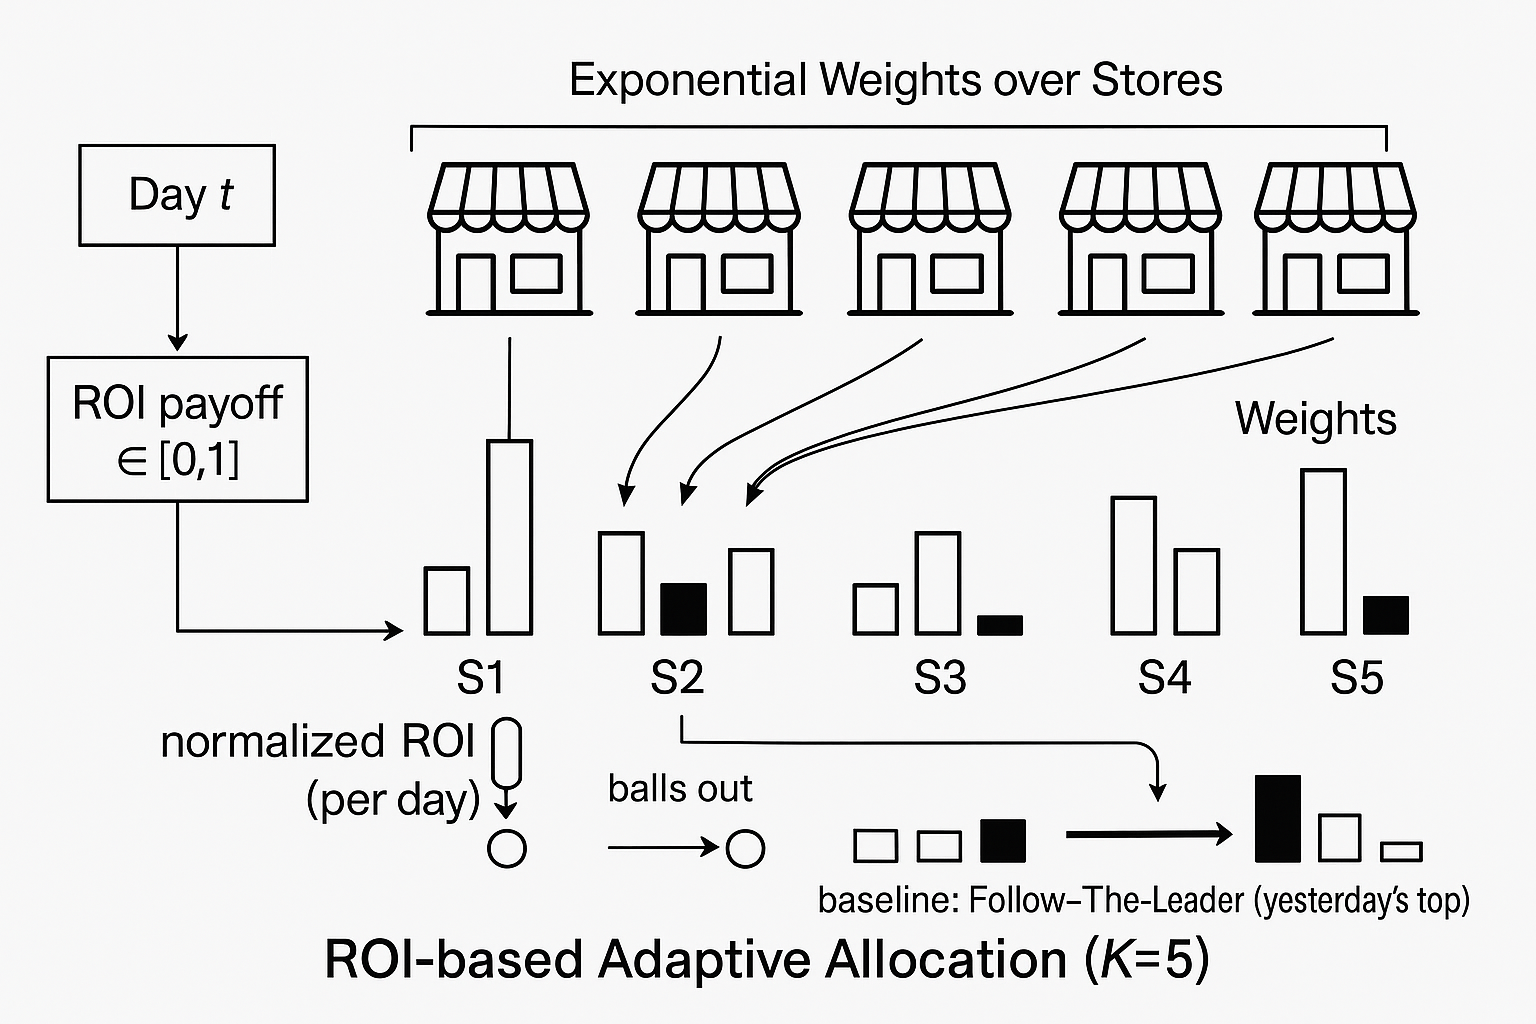
\includegraphics[width=0.4\linewidth]{332Project2/figures/Image_C.png}
    \caption{Image of C}
    \label{fig:placeholder}
\end{figure}

\end{frame}

\begin{frame}{C - Results(Regret)}
\begin{figure}
    \centering
    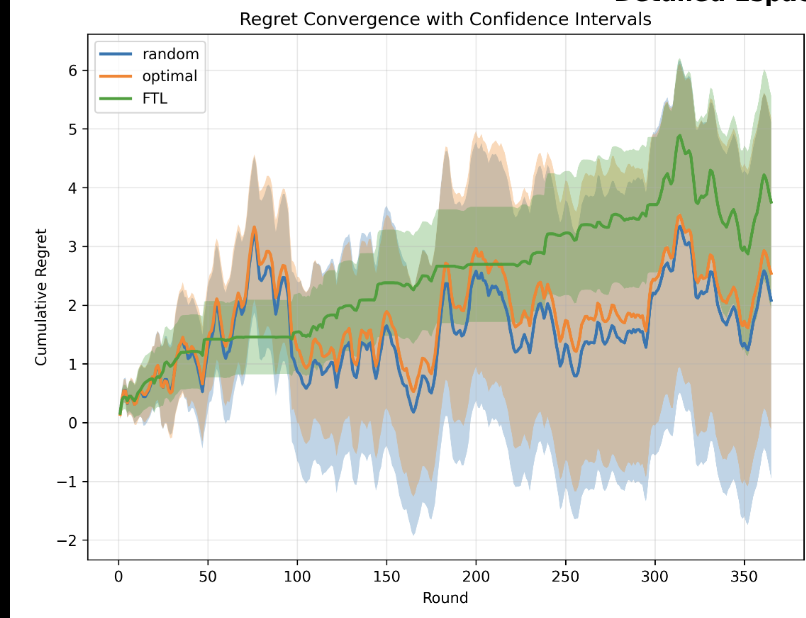
\includegraphics[width=0.5\linewidth]{332Project2//figures/Regret.png}
    \caption{Regret}
    \label{fig:placeholder}
\end{figure}
    
\end{frame}


\subsection{D : RP}

\begin{frame}{D - Motivation}
I have two motivations(both technical and private) to formulate a new data generating model.
    \begin{itemize}
        \item \textbf{Technical} : N-dimensional maximization
        \begin{itemize}
            \item In simple setting, "arm" is one-dimensional. Motivated by prpblem set 3 problem 1, we extend it to an N-dimensional maximization(in practice N=20).
        \end{itemize}
        \item \textbf{Private} : My experience as Research Assistant
        \begin{itemize}
            \item In research, we have to review lots of previous research papers not knowing the whole picture of the field. We have to distribute effort to each papers, which sometimes are trash for your research, sometimes are treasure for your research.
        \end{itemize}
    \end{itemize}
\end{frame}


\begin{frame}{D - Techniques}
    In academic world, there are two often-said characteristics
    \begin{itemize}
        \item \textbf{High-quality papers are mass-produced by a cluster of researchers}
        \begin{itemize}
            \item we can formulate this by introducing correlation of paper's value in a cluster
            \item which disturbs uniform guessing to be optimal and to converge to the no-regret condition
        \end{itemize}
        \item \textbf{Frequent innovations (regime changes) in research methods}
        \begin{itemize}
            \item we can formulate this by introducing possibility of regime changes 
            \item which disturbs FTL to be optimal and to converge to the no-regret condition
        \end{itemize}
    \end{itemize}
    Our technique leverages these well-known properties to formulate online learning in a way that suits the conditions of our problem.
\end{frame}

\begin{frame}{D - Model}
Here is our model.
\begin{itemize}
    \item The research world is divided into several \textbf{clusters of researchers} 
          (e.g., MIT, Stanford, Northwestern).
    \item Each cluster represents a correlated set of ideas or papers whose values
          move together (\textbf{intra-cluster correlation}).
    \item At every round, the researcher distributes total effort 
          across candidate papers:
          \[
          \sum_{i=1}^{N} w_{i,t} = 1, \quad w_{i,t} \ge 0.
          \]
    \item The payoff is the weighted sum of paper values:
          \[
          U_t = \alpha_t^{\mathsf{T}} w_t.
          \]
\end{itemize}
\end{frame}

\begin{frame}{D - Model}
    \begin{block}{Regime Dynamics}
    \begin{itemize}
        \item At any time, one cluster becomes \textbf{hegemony} (high valuation).
        \item The dominant cluster changes according to a \textbf{Markov transition} with probability p:\\
        for example, p = 0.7, 
              \[
              \Pr(z_t = z_{t-1}) = 0.7, \quad 
              \Pr(z_t \neq z_{t-1}) = 0.3.
              \]
        \item In each regime:
              \begin{itemize}
                  \item One cluster has \textbf{High values} ($[0.7, 1.0]$)
                  \item Another has \textbf{Middle values} ($[0.5, 0.8]$)
                  \item Others remain \textbf{Low values} ($[0.0, 0.4]$)
              \end{itemize}
    \end{itemize}
    \end{block}
\end{frame}


\begin{frame}{D - Setting}
    In each round i, 
    \begin{itemize}
        \item There is hidden(unobserved) regime in each round.
        \item The researcher observes the clusters and origin clusters of candidate papers 
        \item The researcher chooses an \textbf{effort allocation vector}
              \[
              w_t = (w_{t,1}, \ldots, w_{t,k}), 
              \quad \text{such that } \sum_{j=1}^{k} w_{t,j} = 1,\; w_{t,j} \ge 0.
              \]
        \item The payoff is computed as a linear combination:
              \[
              U_t = \alpha_t^{\mathsf{T}} w_t.
              \]
    \end{itemize}
\end{frame}

\begin{frame}{D - Interpretation}
    \begin{block}{Interpretation}
    \begin{itemize}
        \item This describes a sequential allocation game:\\
              the researcher gradually redistributes effort across actions
              based on past observed values.
        \item The environment is non-stationary because
              the payoff structure changes due to regime shifts.
        \item The learning algorithm (Exponentiated Gradient)
              adjusts $w_t$ over time to minimize cumulative regret.
    \end{itemize}
    \end{block}
\end{frame}

\begin{frame}{D - Appendix (Example)}
\scriptsize
\textbf{Example Setting}
    \begin{itemize}
        \item Imagine three major research clusters:
              \textbf{MIT}, \textbf{Stanford}, and \textbf{Northwestern}.
        \item Each cluster represents a group of researchers 
              whose papers are highly correlated in value (citations, attention, or impact).
        \item The researcher (our agent) allocates research effort
              across papers from these clusters every round.
    \end{itemize}
\textbf{Regime-Dependent Dominance}
\begin{itemize}
        \item At one period, the \textbf{MIT cluster} becomes dominant 
              --- its papers are cited frequently, gaining high valuation.
        \item Over time, attention shifts:
              Stanford’s ideas rise in popularity,
              then Northwestern takes the lead.
        \item These shifts occur through a stochastic 
              \textbf{Markov regime transition}, 
              creating a dynamic environment.
    \end{itemize}
\textbf{Researcher’s Behavior}
\begin{itemize}
        \item In each round, the researcher chooses how to distribute effort:
              \[
              w_t = (w_{\text{MIT}}, w_{\text{Stanford}}, w_{\text{Northwestern}}),
              \quad \sum w_t = 1.
              \]
        \item The payoff is the weighted performance of papers:
              \[
              U_t = \alpha_t^{\mathsf{T}} w_t.
              \]
        \item As the dominant cluster changes, the researcher must 
              continuously reallocate effort to follow the new trend.
\end{itemize}
\end{frame}

\begin{frame}{D- Appendix (Algorithm in the real world)}
\scriptsize
\textbf{1. Follow-The-Leader (FTL)}
    \begin{itemize}
        \item \textbf{Intuitive meaning:}
              \begin{itemize}
                  \item “MIT is the most famous and successful group — 
                        just follow their papers.”
                  \item Represents a researcher who always trusts 
                        the cluster that has performed best in the past.
              \end{itemize}
        \item \textbf{Problem:} 
              When regimes shift (e.g., attention moves from MIT to Stanford),
              FTL reacts too slowly and suffers large regret.
    \end{itemize}
\textbf{2. Uniform Guessing}
    \begin{itemize}
        \item \textbf{Intuitive meaning:}
              \begin{itemize}
                  \item “Every cluster might have something interesting —
                        I’ll pick papers at random.”
                  \item Represents an exploratory but non-learning researcher.
              \end{itemize}
        \item \textbf{Problem:} 
              Ignores structure and fails to exploit high-performing clusters.
    \end{itemize}
\textbf{Summary about Algorithms}
    \begin{itemize}
        \item Both FTL and Uniform Guessing resemble 
              intuitive human search behaviors in academia.
        \item FTL overfits to the past (conservative imitation),
              while Uniform Guessing underfits (pure exploration).
    \end{itemize}
\end{frame}

\begin{frame}{D - Compare EG and EW}
\textbf{Extension}
    \begin{itemize}
        \item The \textbf{Exponential Weights (EW)} algorithm updates 
              a probability vector over discrete actions:
              \[
              w_{t+1,i} 
              = 
              \frac{
                  w_{t,i} \exp(\varepsilon \alpha_{t,i})
              }{
                  \sum_{j=1}^{k} w_{t,j} \exp(\varepsilon \alpha_{t,j})
              }.
              \]
        \item EW assumes a \textbf{finite action set} and interprets weights as probabilities.
    \end{itemize}
\textbf{Exponentiated Gradient (EG)}
    \begin{itemize}
        \item EG generalizes EW to an \textbf{$N$-dimensional continuous decision space}.
        \item The parameter vector $w_t \in \Delta^N$ represents 
              a continuous allocation (effort, attention, or resource):
              \[
              w_{t+1}
              = 
              \frac{
                  w_t \odot \exp(\varepsilon \nabla_t)
              }{
                  \|\,w_t \odot \exp(\varepsilon \nabla_t)\|_1
              },
              \quad
              \nabla_t = \alpha_t = \frac{\partial U(w_t)}{\partial w_t}.
              \]
    \end{itemize}
\end{frame}

\begin{frame}{D - Game structure and Intuition}
Here's our intuition:
\begin{itemize}
    \item FTL and uniform guessing will both work similarly to typical behaviors of researchers in the real world who choose the leading university (FTL) or collect from any/all universities (uniform random guessing).
    \item Between FTL and random guessing, maybe there is an optimal learning rate
\end{itemize}
\end{frame}

\begin{frame}{D - Results(Regrets)}
\begin{figure}
    \centering
    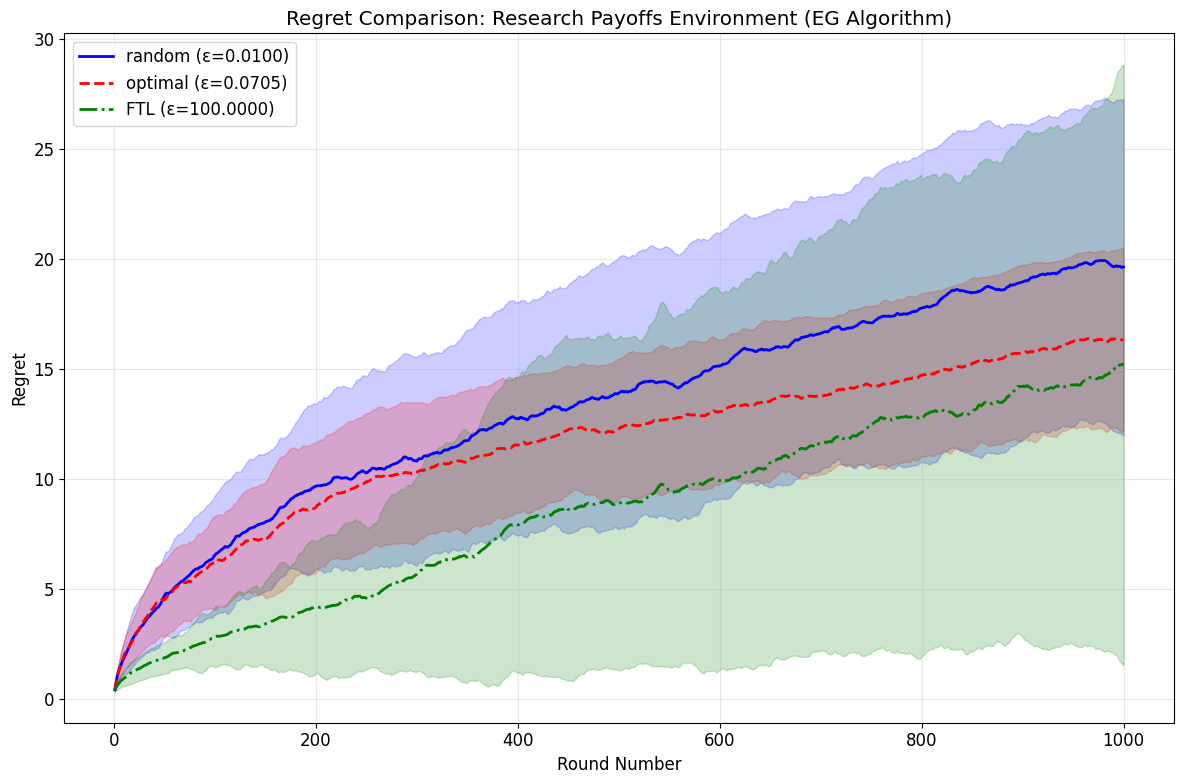
\includegraphics[width=0.5\linewidth]{332Project2/figures/RP_regret.png}
    \caption{Payoff}
    \label{fig:placeholder}
\end{figure}
    
\end{frame}

\begin{frame}{D - Results(Payoffs)}
\begin{figure}
    \centering
    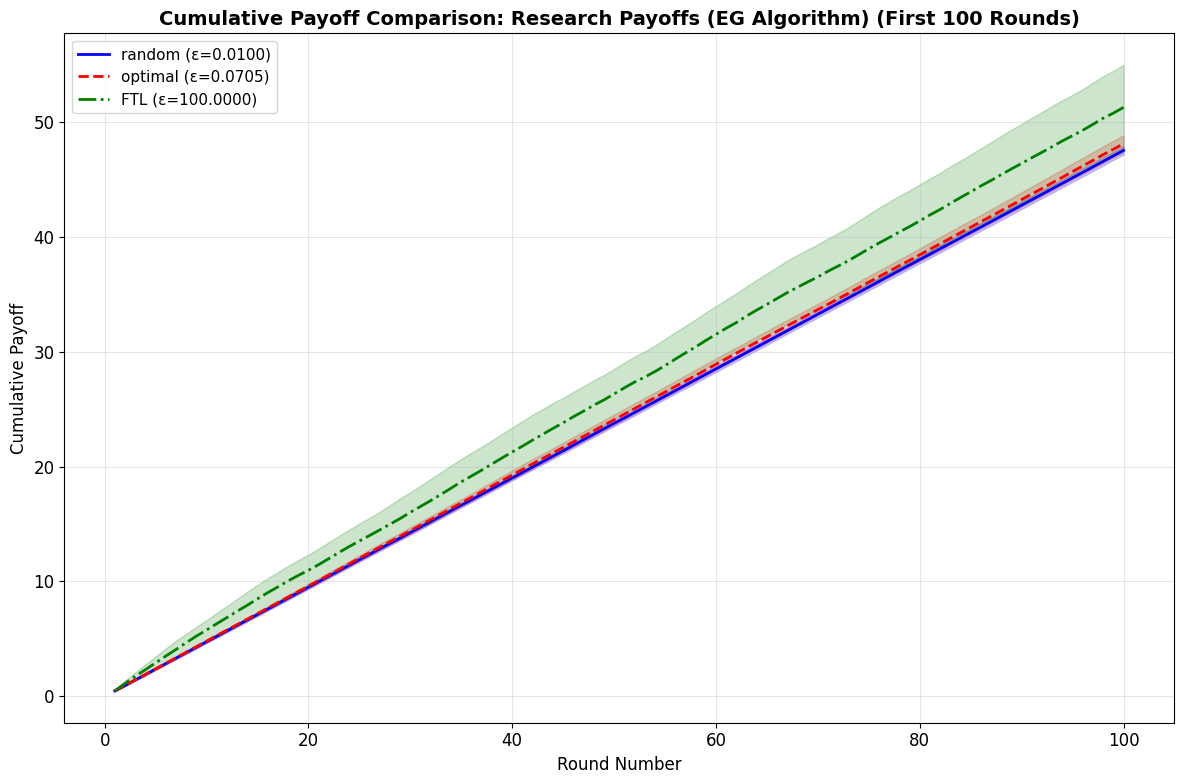
\includegraphics[width=0.5\linewidth]{332Project2/figures/RP_payoff.png}
    \caption{Payoff}
    \label{fig:placeholder}
\end{figure}
    
\end{frame}

\begin{frame}{D - Results(Regret bound)}
\textbf{Results}\\
    According to the setting, regret bound for optimal learning rate is
    \[
    Regret_t \leq 2 * 1 * \sqrt{1000log3} \approx 110
    \]
\end{frame}

\section{Reference and Usage of AI}

\begin{frame}{Reference and Usage of AI}
\begin{itemize}
    \item Data source used in this study is listed below.
    \begin{itemize}
        \item \textbf{Pachinko store data:} Daily store-level ``balls in/out'' statistics obtained from \emph{SloRepo} (\url{https://slorepo.com}), a public repository that compiles pachinko hall data. Data were accessed on October 22, 2025 (America/Chicago). 
    \end{itemize}

    \item AI assistance was used for coding and figure generation;\\
    final verification, interpretation, and responsibility rest with the authors.
\end{itemize}
\end{frame}

\end{document}
